\documentclass[a4paper,11pt,parskip=half,headings=small,DIV=11,notitlepage,abstract=on]{scrartcl}
% This file contains configuration shared between main file and figures

\usepackage{pifont}
\usepackage{xspace}
\DeclareUnicodeCharacter{2460}{\ding{172}\xspace}
\DeclareUnicodeCharacter{2461}{\ding{173}\xspace}

\usepackage{tikz}

\definecolor{HB9UFblue}{RGB}{0,61,165}
\definecolor{HB9UFred}{HTML}{ED135A}

\newcommand{\Ohm}{$\Omega$\xspace}


\newcommand{\uline}[1]{%
  \tikz[baseline=(todotted.base)]{
      \node[inner sep=1pt,outer sep=0pt] (todotted) {#1};
      \draw[color=HB9UFblue,thick] (todotted.south west) -- (todotted.south east);
  }%
}%
                           
\newcommand{\udash}[1]{%
  \tikz[baseline=(todotted.base)]{
      \node[inner sep=1pt,outer sep=0pt] (todotted) {#1};
      \draw[dashed,color=HB9UFred,thick] (todotted.south west) -- (todotted.south east);
  }%
}%

\usepackage{scrlayer-scrpage}
\usepackage{graphicx}
\usepackage{amsmath}
\usepackage[pdfauthor={},pdftitle={},pdfstartview=FitH,pdfborder={0 0 0}]{hyperref}
\usepackage[utf8]{inputenc}
\usepackage{textcomp}
\renewcommand{\thesection}{\Alph{section}}
\renewcommand*{\theenumi}{\thesection.\arabic{enumi}}

\usepackage{ngerman}
\ifoot{\texttt{}}
\ofoot{\texttt{}}

\addtolength{\textheight}{10mm}
\title{Posten C\\Impedanztransformatoren und Mantelwellensperren (``Baluns'')}
\author{}
\date{}
\pagestyle{empty}
\renewcommand*{\titlepagestyle}{empty}
\sloppy

\begin{document}
\maketitle
\vspace{-2cm}

An diesem Posten charakterisierst du die Eigenschaften von Mantelwellensperren
und Impedanztransformatoren. Diese Bauelemente werden oft unter dem Begriff
``Balun'' zusammengefasst -- vermutlich, weil beide durch Bewickeln von
Ringkernen implementiert werden können. Tatsächlich haben diese beiden
Bauelemente aber ganz unterschiedliche Aufgaben: Impedanztransformatoren dienen
dazu, eine Impedanz zu einer anderen zu transformieren (z.B. die
Fusspunktimpedanz einer Antenne zur Impedanz der Speiseleitung),
Mantelwellensperren hingegen dienen dazu, Mantelwellen auf der äusseren Seite
des Schirms von Koaxialkabeln zu unterbinden.

\section{Mantelwellensperren}
Für die Charakterisierung einer Mantelwellensperre wird die Leitung an beiden
Enden kurzgeschlossen und das Bauteil mit einer Transmissionsmessung
ausgemessen (Trace-Format ``LogMag''). Je nach Implementierung der
Mantelwellensperre kann dies folgendermassen geschehen:

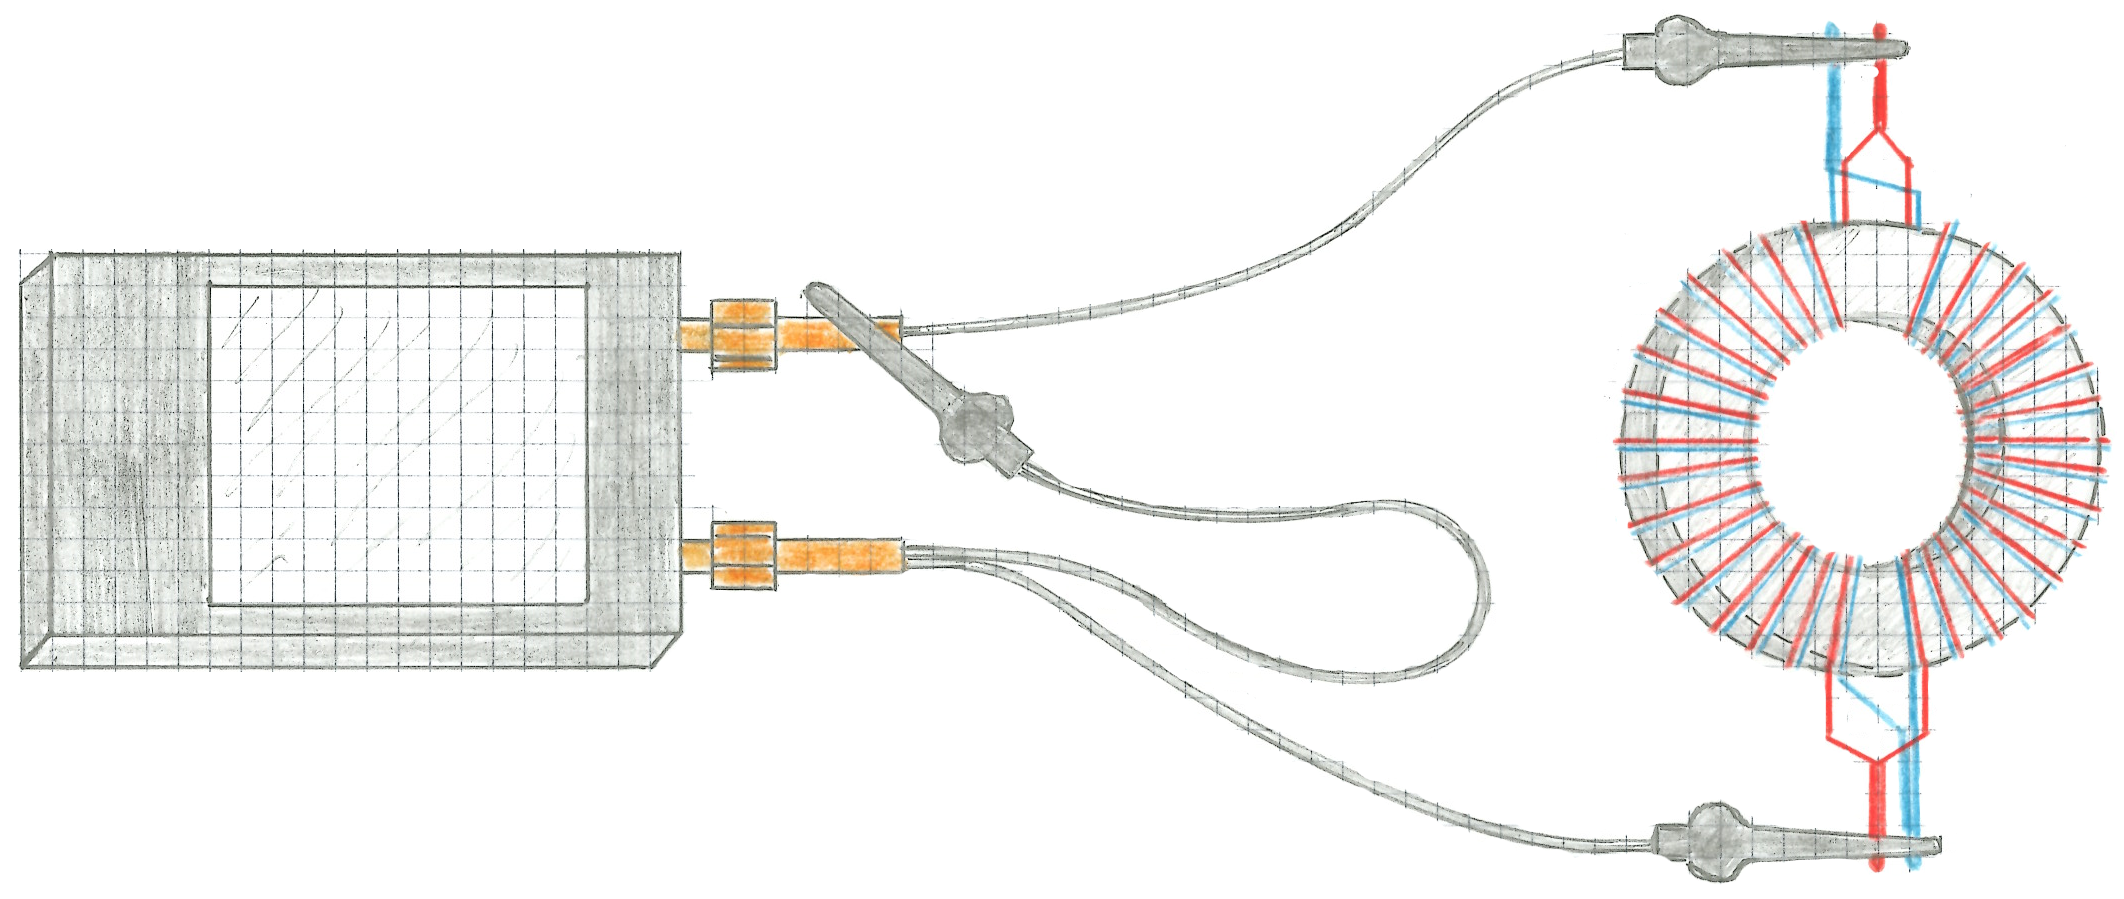
\includegraphics[height=3.5cm]{../skript/figures/illustration_DG0SA.png}\hfill
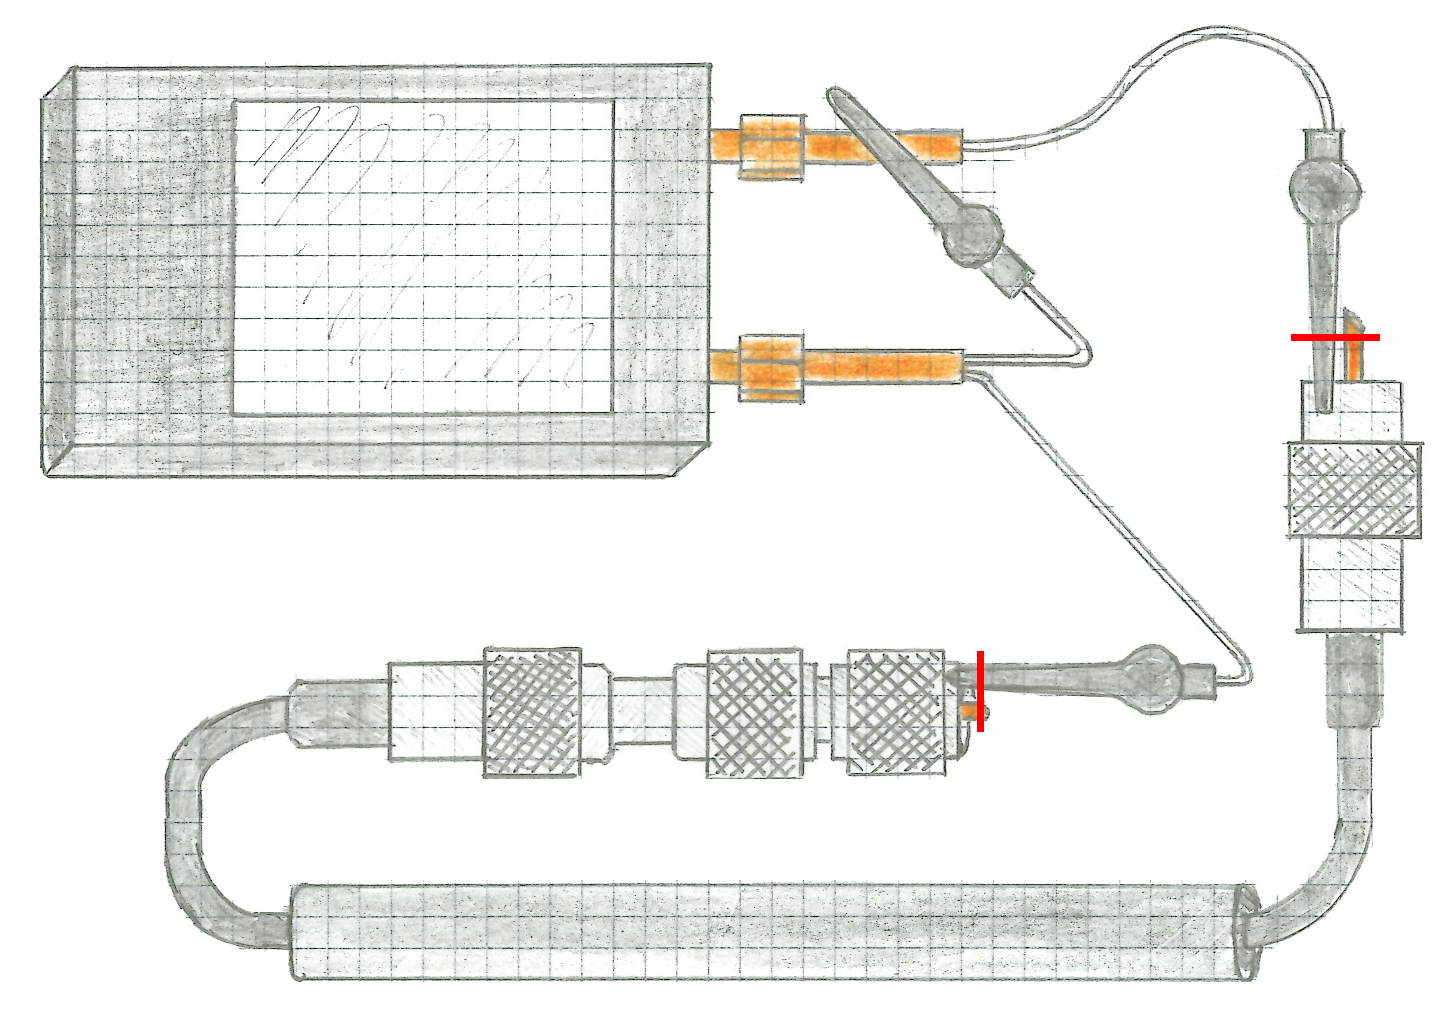
\includegraphics[height=3.5cm]{../skript/figures/illustration_w2du_short.png}

Je nach Situation gibt es unterschiedliche Anforderungen an die
Mantelwellensperre, so dass keine allgemeine minimale Anforderung an die
Dämpfung angegeben werden kann. Davon ungeachtet geben die Lehrbücher eine
minimale Dämpfung von 30~dB als wünschenswert an. Es ist schwierig, eine
Mantelwellensperre zu konstruieren, welche über einen grossen Frequenzbereich
hinweg eine gute Dämpfung aufweist. Deshalb lohnt es sich, selbstgebaute und
auch im Handel erworbene Mantelwellensperren im Bereich der Betriebsfrequenz zu
testen.

Es stehen an diesem Posten verschiedene Mantelwellensperren für eine
Charakterisierung im Frequenzbereich zwischen 1~MHz und 50~MHz bereit: Bauart
nach DG0SA, Bauart nach W2DU, Bauart ``Joghurtbecher'' und ein lose
aufgewickeltes Koaxialkabel. Welche Mantelwellensperre ist für welchen
Frequenzbereich geeignet? Welche sind breitbandig, welche schmalbandig?

\section{Impedanztransformatoren}
Impedanztransformatoren setzen eine Impedanz $Z_1$ in eine andere Impedanz $Z_2$ um.
Dies ist beispielsweise nützlich, wenn die Impedanz einer Antenne auf diejenige
der Speiseleitung transformiert werden soll. Konkret: Eine Endgespiesene Antenne
weist eine Fusspunktimpedanz von mehreren k\Ohm auf; bei der Speisung mit einem
Koaxialkabel mit 50~\Ohm ist eine Impedanztansformation notwendig. Ansonsten würde
der Grossteil der Sendeleitung am Antennenfusspunkt reflektiert, statt von der
Antenne aufgenommen werden. Bei der Spezifizierung des Transformators wird in der
Regel das Impedanzverhältnis $Z_1:Z_2$ oder das Windungsverhältnis $W_1:W_2$ angegeben.
Ersteres ist bei einem einfachen Transformator das Quadrat des letzteren.

Es gibt mehrere Methoden, um Impedanztransformatoren zu charakterisieren: Zunächst
kann der Transformator auf der einen Seite mit der passenden Impedanz abgeschlossen
und dann mit einer Reflexionsmessung geprüft werden (Abbildung links). Dabei ist eine
möglichst gute Rückführungsdämpfung -- also weit weg von 0~dB -- wünschenswert. Bei
dieser Messart ist allerdings nicht klar, ob die nicht zurückgeführte Leistung im
Transformator oder im Abschluss dissipiert wird.

Wenn zwei baugleiche Transformatoren zur Verfügung stehen, dann können diese
zusammengeschaltet und mit einer Transmissionsmessung geprüft werden: Der erste
Transformator wandelt die $Z_1=$50~\Ohm Systemimpedanz auf eine andere Impedanz
$Z_2$ um, der zweite Transformator wandelt diese Impedanz dann wieder zurück
nach $Z_1$ um, wie der rechte Teil der Abbildung zeigt:

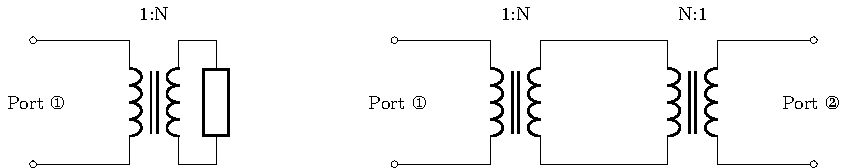
\includegraphics[width=\textwidth]{../skript/figures/transformer/transformer.pdf}\hfill

Im Idealfall ist eine Einfügedämpfung von 0~dB zu erwarten. Alle Verluste entstehen
theoretisch zur Hälfte in je einem Transformator. Oft verfügt man aber nur über einen
Transformator. In diesem Fall kann die Fehlanpassung berechnet und als Referenzwert
hergenommen werden. Beispiel: Ein Transformator mit einem Impedanzverhältnis von 1:4
setzt die Systemimpedanz von 50~\Ohm auf eine Impedanz von 200~\Ohm bzw. 12.5~\Ohm
um, je nachdem, in welche Richtung er beschaltet wird. Dies entspricht einem SWR von
1:4 und, gemäss einschlägiger Rechenprogramme\footnote{\url{https://chemandy.com/calculators/return-loss-and-mismatch-calculator.htm}},
einer Dämpfung von 1.94~dB. Im Idealfall wird die Transmissionsmessung also eine
Dämpfung von 1.94~dB aufweisen, und jede weitere Dämpfung ist auf Abweichungen von
den Idealannahmen zurückzuführen. Vorsicht: Alle beschriebenen Messungen erfolgen bei
geringer Leistung und bilden deshalb Effekte, die bei Sättigung und/oder Erwärmung
der Transformatorkerne erscheinen, nicht korrekt ab.

Zwei Transformatoren mit Impedanzverhältnis 1:4 steht zur Charakterisierung zur
Verfügung. Wähle eine geeignete Messmethode aus und messe den Transformator aus.
Für welchen Frequenzbereich ist er geeignet? Spielt die Orientierung bei der Messung
eine Rolle?
\end{document}
